\scanpage{77}
/ positive Hermitian operators, finally satisfies formula (12).

\margin{\uline{Put 2 and corollary at the beginning}}

\uline{Proposition 3} Let $E$ and $F$ be two Hilbert spaces, let $u_i$ ($i=1,\mathord{.}\,\mathord{-}n$) be Fredholm maps from $E$ to $F$; then $u_1\wedge\mathord{-}\wedge u_n$ is a Fredholm map from $\overset{n}{\Lambda}^{(2)}E$ to $\overset{n}{\Lambda}^{(2)}F$, and
\reversemarginpar\margin{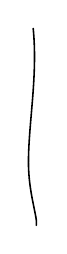
\begin{tikzpicture}[x=1mm,y=1mm,line cap=round]\draw[line width=.2mm] (.8,25) .. controls (1.4,19) and (.2,13) .. (.2,8) .. controls (.2,4) and (1.4,1) .. (1.2,0);\end{tikzpicture}}\normalmarginpar

\[
\begin{array}{@{}l@{\qquad}l@{}}
(13) & {\color{red}\boxed{\color{black}\displaystyle \lVert u_1\wedge\mathord{-}\wedge u_n\rVert_1\leq\frac1{n!}\lVert u_1\rVert_1\mathord{-}\lVert u_n\rVert_1}}
\end{array}
\]

Indeed, it suffices to \deleted{\unsure{$\leq$}} verify \deleted{that if} if \deleted{$u_1=a_1'\otimes$} $u_i=\bar b_i\otimes a_i$, \deleted{\unsure{the} \illegible{1}} with $\lVert\bar b_i\rVert\leq1$, $\lVert a_i\rVert\leq1$, then $\lVert u_1\wedge\mathord{-}\wedge u_n\rVert_1\leq1/n!$, \deleted{\unsure{for}} since then there exists an \unsure{$n$ times|of Ban} linear \deleted{\unsure{continuous}} map \inserted{of norm $\leq1/n!$} from $(\bar E\widehat{\otimes}E)^n$ into \deleted{\unsure{into}} $\bar F\widehat{\otimes}F$ (where $F=\overset{n}{\Lambda}^{(2)}E$) which coincides with \inserted{$(u_1,\mathord{.}\,\mathord{-}u_n)\longrightarrow$} $u_1\wedge\mathord{-}\wedge u_n$ for decomposable $u_i$, hence everywhere since the two maps are continuous \deleted{\unsure{by}} in \deleted{\unsure{so far}} as maps, into $L(F)$.

Now for $u_i=\bar b_i\otimes a_i$, we have

\[
\deleted{\unsure{\overset{n}{\Lambda}}}\quad u_1\wedge\mathord{-}\wedge u_n=\frac1{n!}(\bar b_1\wedge\mathord{-}\wedge\bar b_n)\otimes(a_1\wedge\mathord{-}\wedge a_n),
\]

\inserted{(see Chapter I, N\textsuperscript{o} 1, formula (8))} whence

\[
\lVert u_1\wedge\mathord{-}\wedge u_n\rVert_1\leq\frac1{n!}\lVert\bar b_1^c\wedge\mathord{-}\wedge\bar b_n\rVert\,\lVert a_1\wedge\mathord{-}\wedge a_n\rVert\leq\frac1{n!}\prod\lVert a_i\rVert\,\lVert\bar b_i\rVert
\]

(formula (5,), whence (13).

\uline{Corollary 1} Let $E$ be a Hilbert space, and \deleted{\unsure{$u$}}\inserted{$u,u_i$} $\in L^1(E;E)$ \inserted{$(i=1,\mathord{-} n)$} be \deleted{some} Fredholm operators on $E$. Then $\overset{n}{\Lambda}u$ is a Fredholm operator on $\overset{n}{\Lambda}^{(2)}E$, and we have
\reversemarginpar\margin{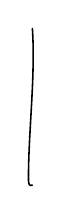
\begin{tikzpicture}[x=1mm,y=1mm,line cap=round]\draw[line width=.2mm] (.7,20) .. controls (1.1,14) and (.2,7) .. (.2,1) .. controls (.2,.1) and (.3,0) .. (.7,.1);\end{tikzpicture}}\normalmarginpar

\[
\begin{array}{@{}l@{\qquad}l@{\quad}l@{}}
(14) & \deleted{\unsure{\text{then}}}\ \deleted{\unsure{\alpha_n(u)}}{\color{red}\boxed{\color{black}\displaystyle\left\{\begin{aligned}
\alpha_n u_1,\mathord{-}u_n)&=\operatorname{Tr}u_1\wedge\mathord{-}\wedge u_n)\\
\alpha_n(u)&=\operatorname{Tr}(\overset{n}{\Lambda}u)
\end{aligned}\right.}} & \begin{array}{@{}l@{}}\strut\\\text{in particular}\end{array}
\end{array}
\]

(where $\alpha_n(u)$ is ${\color{red}\overline{\color{black}\text{defined in}}}$ Chapter 1, \S~2, proposition 1) Indeed, $(14)_{\unsure{2}}$ is true \deleted{for \unsure{every}} when one

\margin{78}
